\newpage
\section{Calculations}

\begin{figure}[!h]
  \centering
  \begin{subfigure}{0.6\textwidth}
    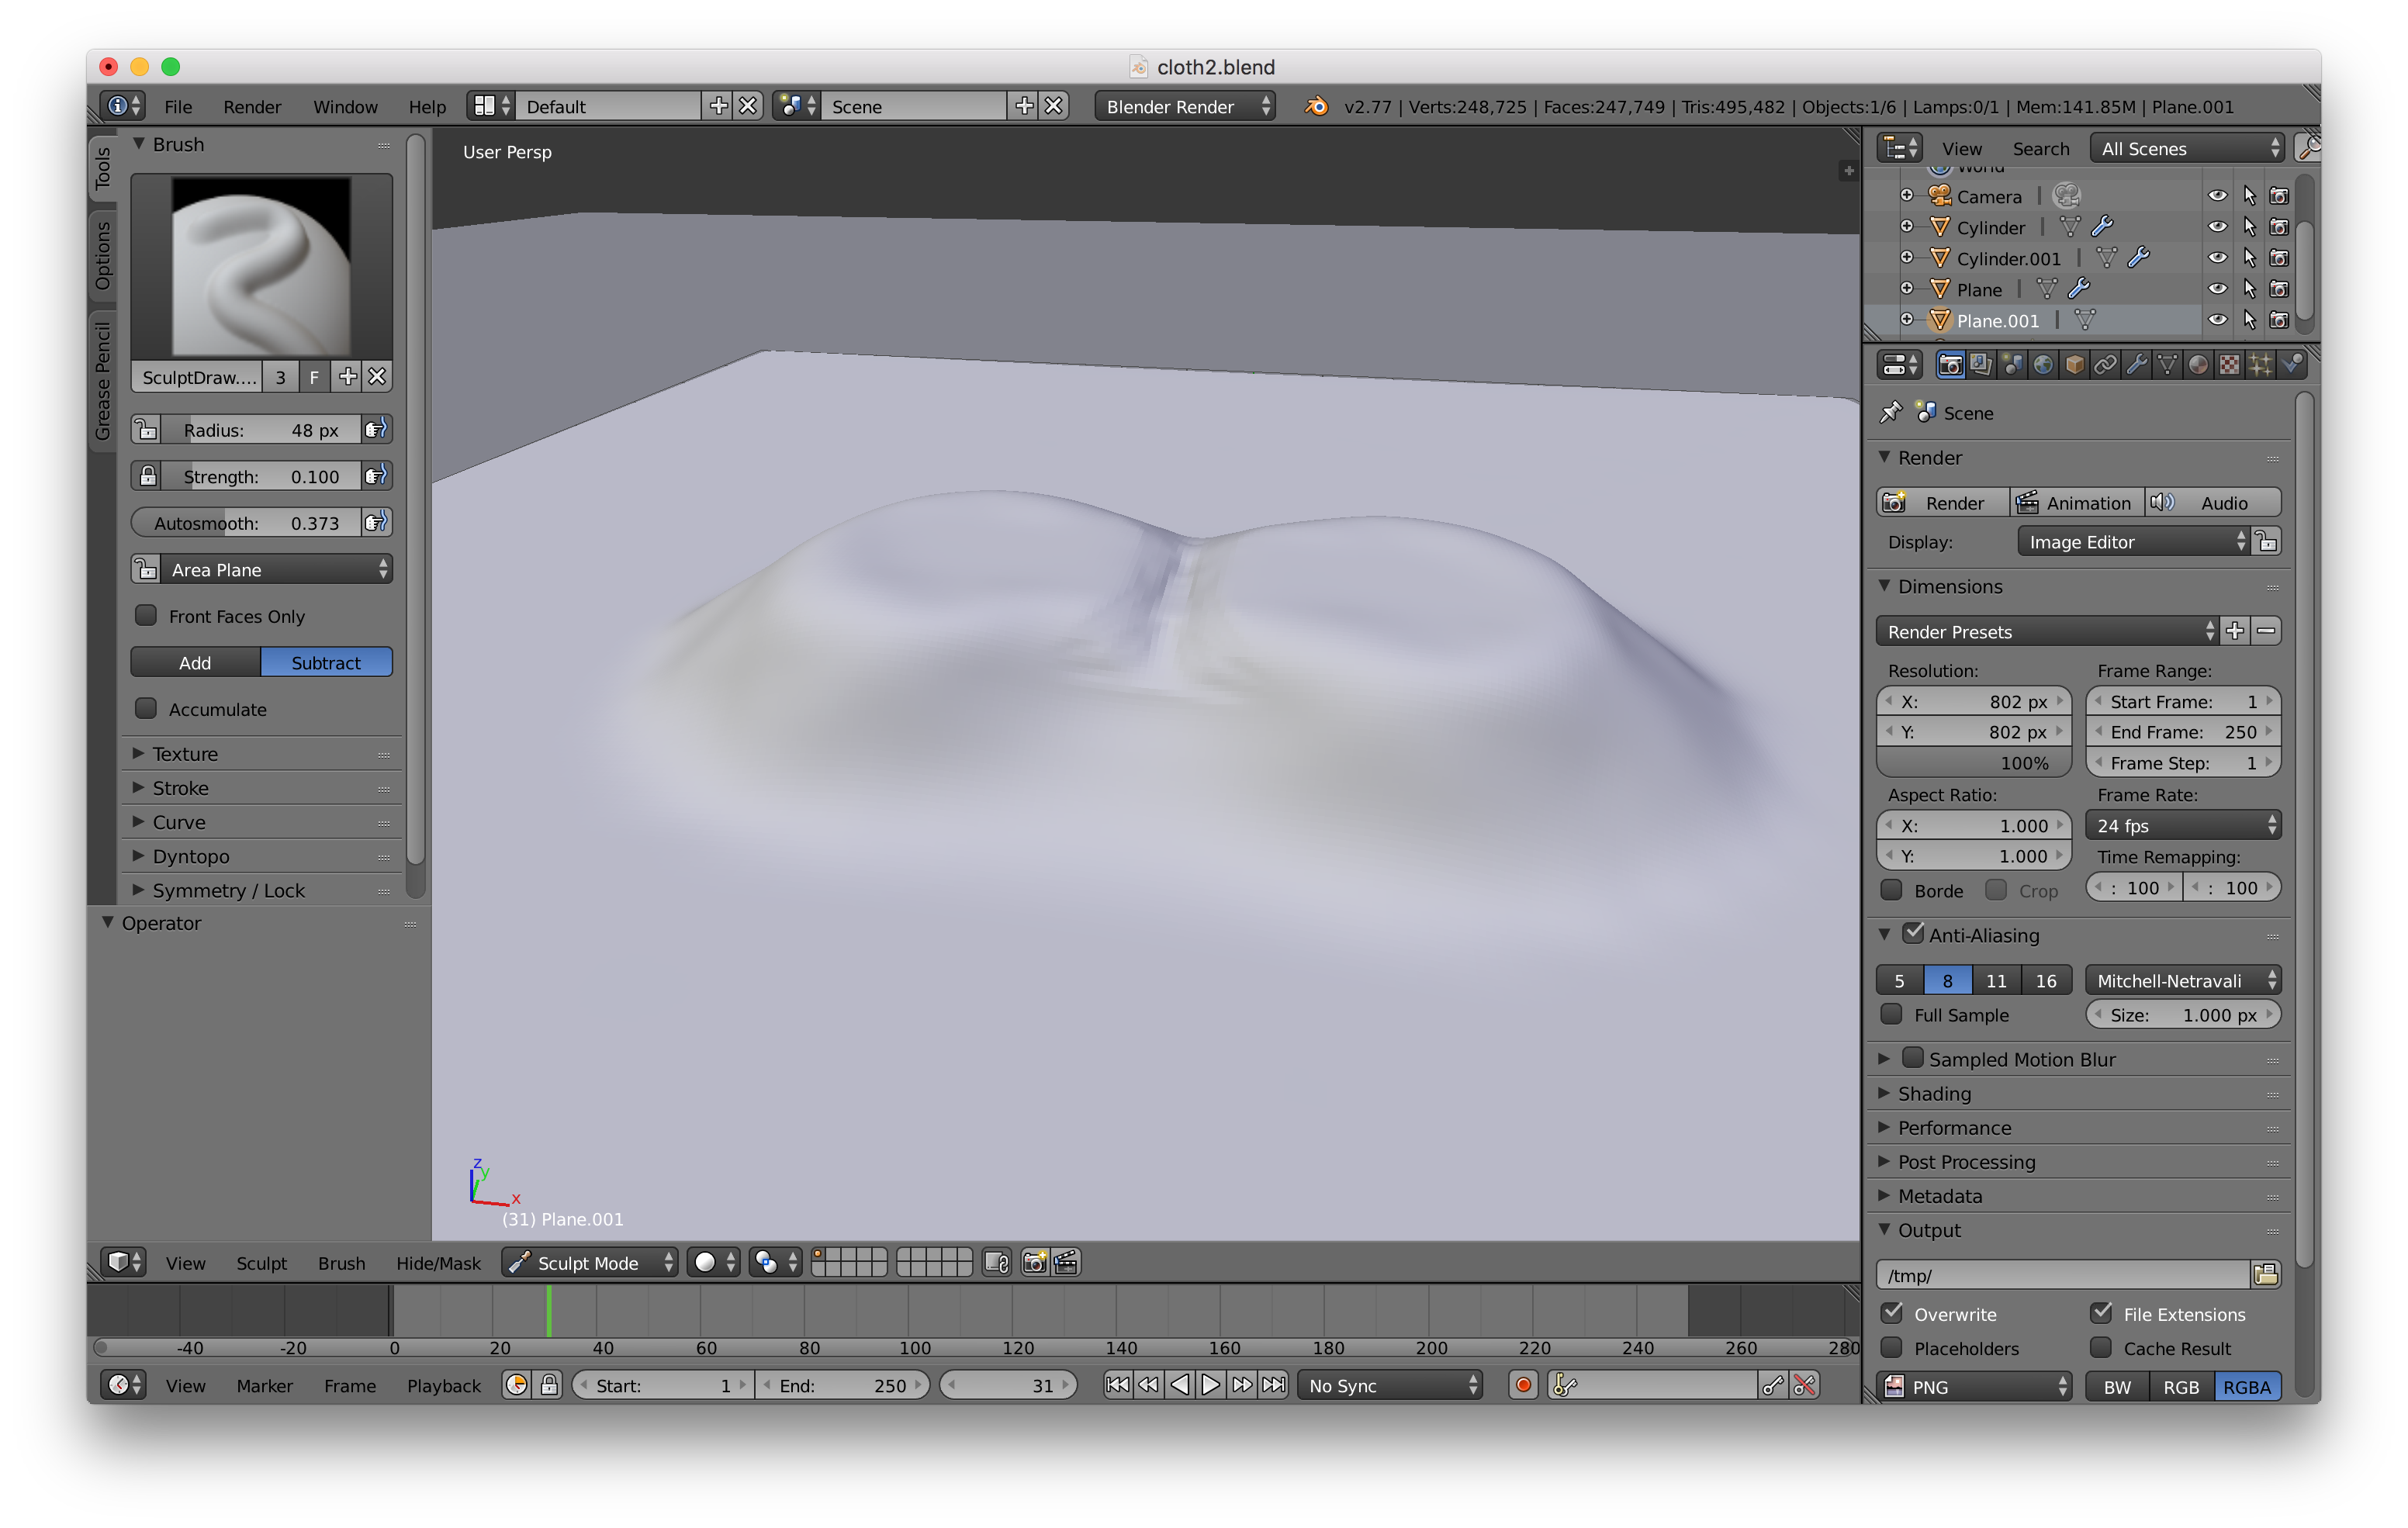
\includegraphics[width=\textwidth]{./images/blender.png}
  \end{subfigure}
  ~
  \begin{subfigure}{0.35\textwidth}
    
\includegraphics[width=\textwidth]{./images/map.png}
  \end{subfigure}
  \caption{\textbf{(a)} Cloth simulation in Blender 2.7. An elastic material is dropped on 2 cylinders with a radius of \SI{50}{nm}. \textbf{(b)} A generated heightmap after rendering. Black corresponds to 0, white to maximum height.}
\end{figure}


\begin{figure}[!h]
  \centering
  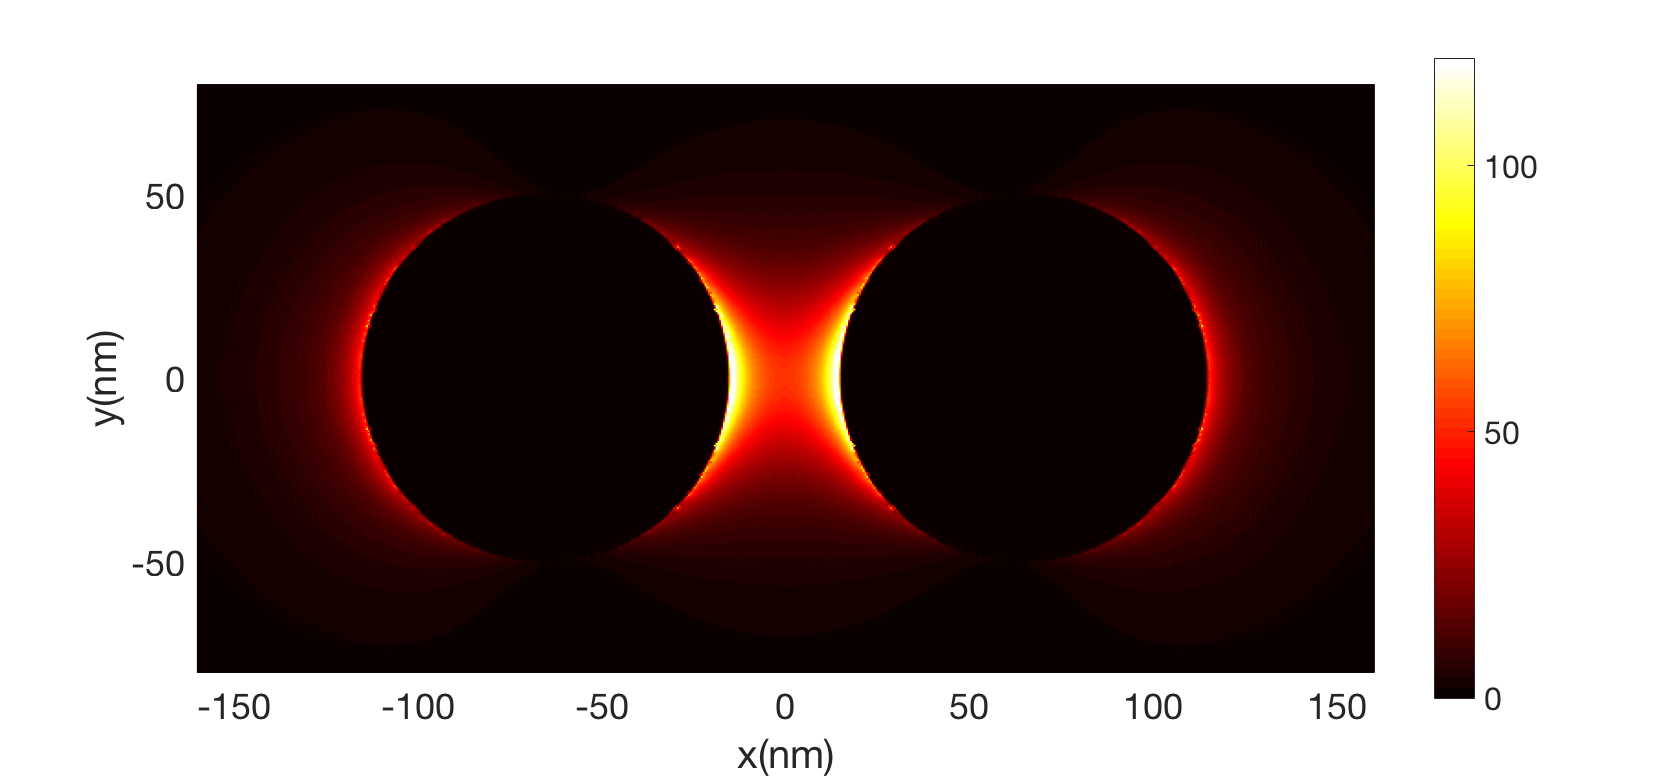
\includegraphics[width=\textwidth]{./images/graphene-layer.png}
  \caption{Near field enhancement $|E/E_0|^2$ in the layer of graphene after applying the height map.}
\end{figure}

\begin{figure}[!h]
  \centering
  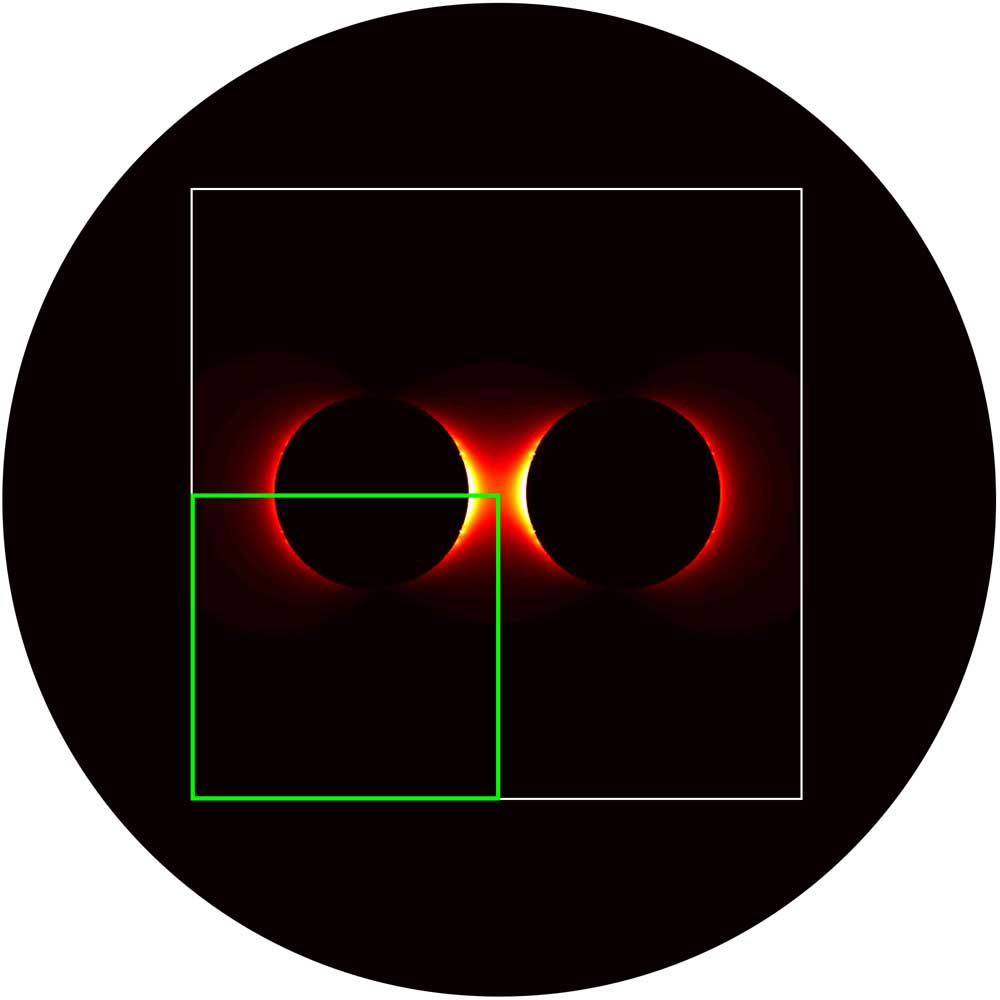
\includegraphics[width=0.5\textwidth]{./images/fwhm-chart.jpg}
  \caption{The simulated square area (green box) compared to the calculated area (white box) compared to the total area measured by the laser (approximated as circle). The laser has a fwhm of \SI{570}{nm} according to \cite{heeg}.}
\end{figure}

\newpage
\null
\newpage
